\section{Laboratory Techniques and Safety}

\begin{multicols}{2}


%\section*{}


\subsection{Display of Hazardous \hfill \\ Chemicals}

\begin{center}
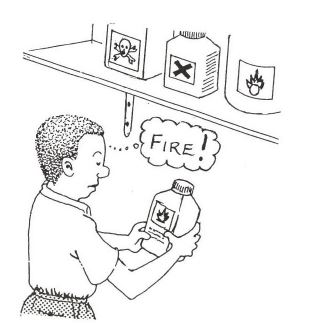
\includegraphics[width=0.45\textwidth]{./img/source/display-chemicals.jpg}
\end{center}

\begin{description*}
%\item[Subtopic:]{}
%\item[Materials:]{}
%\item[Setup:]{}
\item[Procedure:]{Display some well labelled containers with
hazard symbols for the students and let them
talk about them.}
%\item[Hazards:]{}
%\item[Questions:]{}
%\item[Observations:]{}
%\item[Theory:]{}
%\item[Applications:]{}
%\item[Notes:]{}
\end{description*}

\subsection{A Safety Game}

\begin{center}
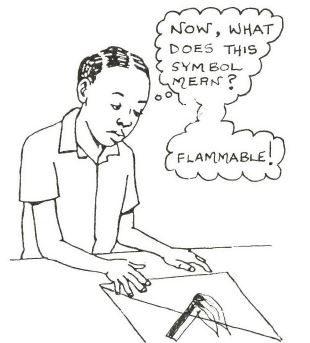
\includegraphics[width=0.45\textwidth]{./img/source/safety-game.jpg}
\end{center}

\begin{description*}
%\item[Subtopic:]{}
\item[Materials:]{Cards of hazard symbols}
%\item[Setup:]{}
\item[Procedure:]{Play a game with the symbol charts. A
student is given a hazard symbol. He has to
explain the hazard shown and to explain the
necessary safety precautions in order to avoid
that hazard.}
%\item[Hazards:]{}
%\item[Questions:]{}
%\item[Observations:]{}
%\item[Theory:]{}
%\item[Applications:]{}
%\item[Notes:]{}
\end{description*}

\columnbreak

\subsection{The Cleanliness Play}

\begin{center}

\includegraphics[width=0.45\textwidth]{./img/source/cleanliness-play.jpg}
\end{center}

\begin{description*}
%\item[Subtopic:]{}
%\item[Materials:]{}
%\item[Setup:]{}
\item[Procedure:]{Ask the students to play group-wise short
and funny scenes using appropriate words to
make them familiar with cleanliness rules.}
%\item[Hazards:]{}
%\item[Questions:]{}
%\item[Observations:]{}
%\item[Theory:]{}
%\item[Applications:]{}
%\item[Notes:]{}
\end{description*}

\subsection{The Tidiness Play}

\begin{center}
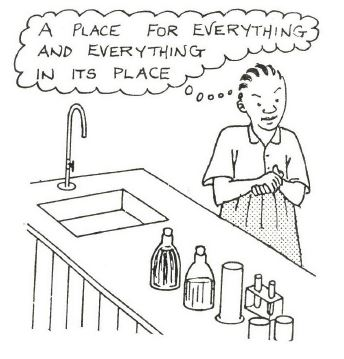
\includegraphics[width=0.45\textwidth]{./img/source/tidiness-play.jpg}
\end{center}

\begin{description*}
%\item[Subtopic:]{}
%\item[Materials:]{}
%\item[Setup:]{}
\item[Procedure:]{Chemists are very tidy. Apparatus and
reagents should be arranged on the table so that
they can be reached easily but at a safe distance
from the experiment.}
%\item[Hazards:]{}
%\item[Questions:]{}
%\item[Observations:]{}
%\item[Theory:]{}
%\item[Applications:]{}
%\item[Notes:]{}
\end{description*}

%==================================================================================================%


\end{multicols}

\pagebreak